% 1.1.ConventionMethod.tex
%	Last update: 2019/07/24 F.Kanehori
%\newpage
\subsection{M6fyRuhEFB7guPkI}
\label{subsec:ConventionalMethod}

\noindent
GitHub\KLUDGE からSpringhead\KLUDGE をダウンロードすると、
\SprLib \KLUDGE をビルドするためのソリューションファイル
\KLUDGE およびプロジェクトファイルがその中に含まれています。

\medskip
\ifLwarp
\Vskip{-.8\baselineskip}
\begin{narrow}[15pt]
	\begin{figure}[h]
	    \begin{center}
	    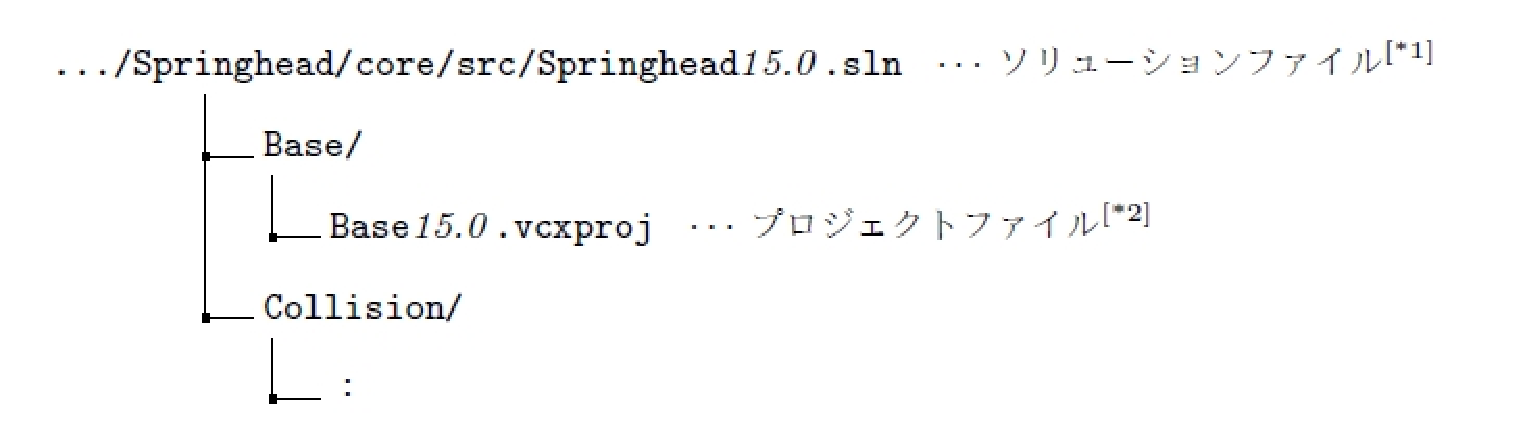
\includegraphics[width=.9\textwidth]{fig/DownloadTree.eps}
	    \end{center}
	    \label{fig:DownloadTree}
	\end{figure}
\end{narrow}
\Vskip{-.8\baselineskip}
\else
\begin{narrow}
    \begin{narrow}[20pt]\begin{minipage}{\textwidth}
	{\footnotesize{\dirtree{%
		.1 \hspace{-10mm}.../Springhead/core/src/Springhead\it{15.0}.sln
			\Anno{\SolutionFile}.
		.2 Base/.
		.3 Base\it{15.0}.vcxproj
			\Anno{\ProjectFile}.
		.2 Collision/.
		.3 \KLUDGE :.
	}}}
	\medskip
  \end{minipage}\end{narrow}
\end{narrow}
\fi

\noindent
\KLUDGE 上記の\SolutionFile \KLUDGE を実行すれば\SprLib \KLUDGE を生成することができ、
\KLUDGE アプリケーションプログラム用のソリューションファイルに
\KLUDGE 上記の\ProjectFile \KLUDGE を\KQuote{\KLUDGE 既存のプロジェクト}\KLUDGE として追加すれば、
\KLUDGE アプリケーションと\SprLib \KLUDGE の開発を同時に行なうことができました。

\KLUDGE 後者の場合は、\ProjectFile \KLUDGE は直接共有されることになります。
\KLUDGE このため、複数のソリューションファイルを同時に開き、あるアプリケーションで
\ProjectFile \KLUDGE に変更が及ぶような修正(\KLUDGE ソースファイルの追加・削除)\KLUDGE を実施しても、
\KLUDGE その変更は他のアプリケーションに直ちに反映されました。
(\KLUDGE プロジェクトが環境外で変更された旨のダイアログが出ます)

\medskip
\noindent
\KLUDGE この方法はうまく機能していますが、次の点が難点として挙げられます。

\Vskip{-.5\baselineskip}
\begin{itemize}
  \item	Visual Studio\KLUDGE のバージョンが変わる度に、
	\KLUDGE ソリューションファイルとプロジェクトファイルを作り直す必要がある。
  \item	Windows\KLUDGE 以外のプラットフォームに対しては、
	Makefile\KLUDGE などを別途作成する必要がある。
\end{itemize}

% end 1.1.ConventionMethod.tex
